\documentclass[11pt]{article}
\renewcommand{\baselinestretch}{1.1}

%%% Add packages here
\usepackage{graphics}
\usepackage{graphicx}
\usepackage{lscape}
\usepackage{amsfonts}
\usepackage{parskip}
\usepackage{amsmath}
\usepackage{amsthm}
\usepackage{amssymb}
\usepackage{latexsym}
\usepackage{color}
\usepackage{verbatim}
\usepackage{fancyhdr}
\usepackage{fancybox}
\usepackage[utf8]{inputenc}
\usepackage{amssymb}
\usepackage{parskip} % for skiping paragraphs
\usepackage{float}
\usepackage{subcaption} % side by side plots


%%%%%%%%%%%%%%%%%%%%%%%%%%%%%%%%%%%%%

%%% Margins
\addtolength{\oddsidemargin}{-.50in}
\addtolength{\evensidemargin}{-.50in}
\addtolength{\textwidth}{1.0in}
\addtolength{\topmargin}{-.40in}
\addtolength{\textheight}{0.80in}

%%% Header
\pagestyle{fancy}
\chead{\groupname}
\rhead{}
\lhead{}
\cfoot{\thepage}
\renewcommand{\headrulewidth}{0.4pt}
%%%%%%%%%%%%%%%%%%%%%%%%%%%%%%%%%%%%%


%%%%%%%%%%%%%%%%%%%%%%%%%%%%%%%%%%%%%%%%%%%%%%%%%%%%%%%%%%%%%%%%%%%%%%%%%%
%%%%%%%%%%%%%%%%%%%%%%%%%%%%%%%%%%%%%%%%%%%%%%%%%%%%%%%%%%%%%%%%%%%%%%%%%%
%%%%%%%%%%%%%%%%%%%%%%%%%%%%%%%%%%%%%%%%%%%%%%%%%%%%%%%%%%%%%%%%%%%%%%%%%%
%%%%%%%%%%%%%%%%%%%%%%%%%%%%%%%%%%%%%%%%%%%%%%%%%%%%%%%%%%%%%%%%%%%%%%%%%%
%%% START MAKING CHANGES HERE!

%%% Group details - PLEASE PUT YOUR GROUP NUMBER HERE!
\newcommand{\groupname}{Term paper: Stochastic Processes (January - 2020) - Group 1}
%%%%%%%%%%%%%%%%%%%%%%%%%%%%%%%%%%%%%

\begin{document}
	\clearpage\thispagestyle{empty}
	
	\begin{center}
		% title
		\textbf{\huge{
				The incremental Cost of HIV patients care in a resource limited setting.
		}} \\[1.5cm]
		% details
		\Large{
			STA 8202: Stochastic Processes \\
			Term paper \\
			January-April 2020\\[0.5cm]
			Master of Science in Statistical Science\\
			Strathmore University	
		}
	\end{center}
	
	\vspace*{1cm}
	\textbf{\large{Group members:}}\\
	Christopher Maronga (122458) \\
	Lilian Sam (124441) \\
	Laban Bore (124270) \\
	Joram Andrew (124765) \\[0.5cm]
	
	\noindent\textit{Submission Date:} TBD
	
	\vspace*{2.5cm}
	\textbf{\large{Lecturer:}}\\
	Dr. Collins Odhiambo 
	
	
	%%% THE WRITTEN PROJECT - MAX. 20 PAGES (everything included)
	%%% page numbering starts here.
	\newpage \setcounter{page}{1}
	
	\begin{abstract}
		\noindent Multi-state Semi-Markov processes are useful tools for studying complex dynamics such as chronic diseases. Laboratory measurement of plasma HIV viral load is used to determine the extent of body immune destruction as well as monitor the disease progression. The World Health Organization (WHO) has put in place clinical staging that uses various clinical parameters to aid in managing the HIV patients. The WHO staging puts both adults and children into 4 hierarchical stages ;stage 1(asymptomatic) to stage 4 (AIDS) depending on viral load suppression and various observable clinical conditions.The aim of this study was to use Semi-Markov chain to determine the cost of keeping patients on WHO stage 1 verse other higher staging.\vspace*{2mm}
		
		\noindent Estimating factors associated with transitions between each stage of progression for chronic diseases, multi-state modeling is highly recommended. The major predictors of the intensity of transitions between different states of HIV patients were DCM, Age group, Sex and DCM status. To predict WHO stages’ cost effectiveness, using semi-Markov concept the HIV viral load was classified as follows; stage 1 $(VL <400$ copies/ml), stage 2 $(400< VL <600)$ and stage 3 $(600<VL< 999)$\vspace*{2mm}
		
		A total of 366 HIV patients were analyzed in this study. 552 transitions between different WHQ stages were observed.
		
		[Brief summary of the results (after analysis) and resolutions to be discussed]
		
	\end{abstract}
	\rule{\textwidth}{0.4pt}
	
	
	\section{Introduction}\label{introduction}
	For more than four decades now, human immunodeficiency virus (HIV) infection has become the epicenter of the diseases challenging humanity and a major focus of public health specialists and researchers. Laboratory measurement of plasma HIV viral load is used to determine the extent of body immune destruction as well as monitor the disease progression. The World Health Organization (WHO) has put in place clinical staging that uses various clinical parameters to aid in managing the HIV patients. The WHO staging puts both adults and children into four hierarchical stages ;stage 1(asymptomatic) to stage 4 (AIDS)depending on viral load suppression and various observable clinical conditions.\\
	
	Increase in viral load values results to an increase of HIV transmission risks. HIV Viral load(VL) is the measure of the number of HIV viruses in the bloodstream majorly measured in milliliter. Patients are put in Differentiated Care Model (DCM) to suppress the patient's VL to undetectable level or a level too low for virus detection by a VL test. Most studies of HIV/AIDS have analyzed the factors associated with therapeutic failure, such as death, opportunistic disease, detect Viral Load (VL) or low levels of immunity, using semi parametric Cox models (Pradeep et al., 2010; Muralidhar et al., 2010; Keiser et al., 2010;Koethe et al., 2010; Neuhaus et al., 2010). From literature the cost effectiveness of viral load monitoring depends on the test prices and rates of virologic failure. Virologic failure would determine the importance of viral monitoring. A higher rate of virologic failure due to low adherence or high resistance rates would result to higher viral load monitoring resulting to higher cost effectiveness ration of viral load testing. \\
	
	%HIV transmission risk increases as viral load values increases. 
	Following 2003 WHO guidelines, the measure of HIV viral load was not recommended for use in a resource limited setting as it was for the high-income counties. This was due to in availability of the equipment's and the high cost of viral test. Since then interventions to cub this challenge where adopted and under 2004 revised WHO guidelines VL testing was available in some resource limited setting. Through available, the challenge is affordability especially for higher stages. For this study DCM follow up was used to help maintain patients in lower stages (stage I). Recent studies have shown that the predicted probability of patients that changing their status given their current state allows the measurements of medical scientific progresses due to the advances in the treatment of the HIV/AIDS (D’Amico et al., 2009). Since the discovery of HIV/AIDS, numerous mathematical models Blasi and Manca (2004) have been developed to describe infectious disease transmission dynamics, understand the mechanisms of epidemic propagation, assess the impact of interventions on public health or forecast the future of epidemics.\\
	
	Numerical analyses of the homogeneous semi-Markov process are dealt by Corradi et al. (2004; Janssen and Manca, 2001). Other more literature include (Davidov and Zelen, 2000; Viladent and Van Ackere, 2007; Satten and Sternberg, 1999; Baryarama et al., 2005). Several researchers have studied Markov processes with covariates and a procedure to obtain the parameters in a model with covariates has been reported For longitudinal chronic disease studies with categorical response variables, the natural development of a chronic disease is often expressed in terms of different states and multistate models are widely used to model the progression of individuals through these states (Goshu and Dessie, 2013).
	\\ 
	
	%The main objective of our study was to investigate the factors associated with HIV disease progression from one stage to another and outline risk factors for immune deterioration in HIV patients using semi-Markov modelling\\
	
	In this study, we will use multi-state semi-Markov process to study the determine factors associated with the progression between different states of HIV.The data was collected from a resource limited setting is used to investigate the factors associated with HIV disease progression from one stage to another using Semi-Markov concept. Additionally, the aim of the study was to outline risk factors for immune deterioration in HIV during the DCM follow-up. The VL of patents was classified as the following, based on the worst of the disease; stage I the Asymptotic stage, stage II thee Mildly Symptomatic Stage and stage III the Moderated Symptomatic Stage. \\
	
	
	\section{Methods and Materials}
	Multistate stochastic models have gained popularity in investigating dynamics of chronic diseases. In this study, we used a homogeneous Semi-Markov model with defined distribution of waiting time, hazard function of waiting and Semi-Markov process. We also had selected covariates in an group of HIV patients. The aim is to analyze the progression of HIV infection through the three WHO stages and evaluate the contribution of the covariates.The covariates under consideration were WHOstaging (stage= 1, stages greater than 1= 0), DCM(yes= 1, No= 0), AgeGroup(adult= 1,child= 0) and Sex(Female= 1, Male= 0)\\
	
	Semi-Markov assumes that the probability of a patient goes to from one state to another is not depend on the past states where a patient was, but depends on the current state.Additionally, probability that a patient jump from one state to another depends on the elapsed time in the current state.The target population for this study is HIV patients under DCM. A total of 366 HIV patients were analyzed in this study. There were 552 transitions between different WHQ stages were observed. The data was assumed to have a Markov property; that is the current and future states depends only on the immediate past and present states respectively. It is also studied under continuous time frame work explaining the use of multi-state model based on Markov process.Continuous homogeneous Semi-Markov model was employed in the analysis. 
	\begin{center}
		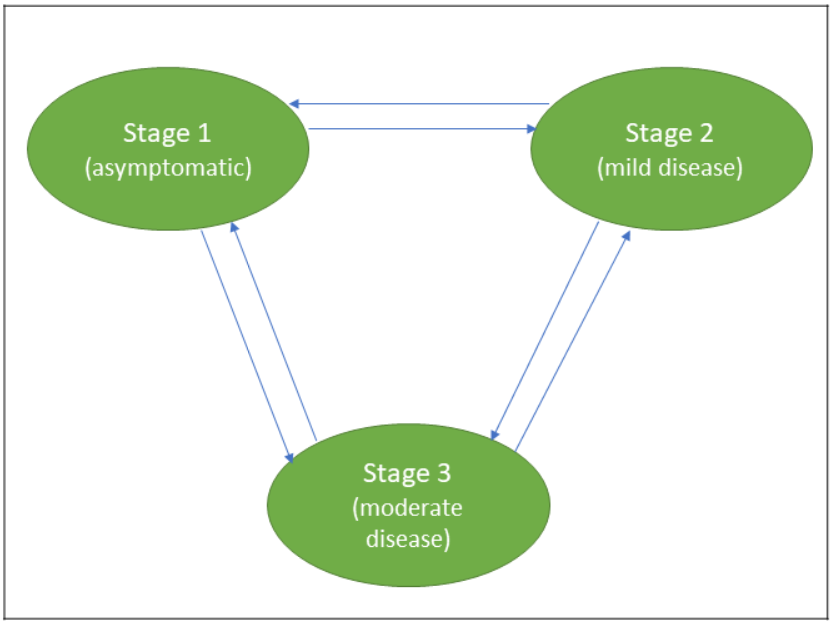
\includegraphics[scale=0.5]{stages}\\
	\end{center}

	%For the effectiveness of our study several distributions were tried, and individual distribution p-values Were keenly examined for significance. Weibull sojourn time distribution was the most appropriate distribution.
	%%and is used as sojourn time distribution under multi-state models.
	It is assumed that process spends some time in a given state and random time has distribution $G_{ij}(x)$,Weibull sojourn time distribution was found to be the appropriate distribution and used as sojourn time distribution and hazard rate distribution under multi-state models. Weibull distribution: The hazard function is defined as 
	$$\displaystyle F_{hj}(t)=\lambda_{hj}\left(\frac{1}{\sigma_{hj}}\right)t^{\lambda _{h j}-1}\,\,t\geq 0,$$
	where  $F_{hj}(x)$ is the measure of patient's likelihood of transiting to next stage at time t. Again, Weibull distribution is used because different values of $\left(\frac{1}{\sigma_{hj}}\right)$ can result to increasing hazard rate$\left(\frac{1}{\sigma_{hj}}>1\right)$, decreasing hazard rate,$\left(\frac{1}{\sigma_{hj}}<1\right)$ or constant hazard rate $\left(\frac{1}{\sigma_{hj}}=0\right)$. 
	Weibull sojourn time is time is defined as 
	$$G_{hj}(t)=1- exp(\sigma^{-1}_{hj}t^{\lambda_{hj}}),\,\, t\geq 0$$
	where $\lambda_{hj}$ determines the shape of hazard rate function and how $\sigma^{-1}_{hj}$ can be varied. 
	\label{methods}
	
	
	
	\section{Result}\label{result}
	Data containing total of 366 HIV patients was analysed in this study. 552 transitions between different WHO stages were observed with an assumption of no transition within same state. 
	
	The study comprised of 209 male patients and 157 female patients. 42\% of the patients were under differentiated care model and a majority were adults (94\%) Table \ref{my_table}
	
\begin{table}[H]
	\centering
	\caption{Patient Baseline Characteristics}
	\label{my_table}
	\begin{tabular}{|l|c|} % arguments to define the alignment of contents of the table, borders
		\hline
		Characteristics & \\
		 \hline 
		\textbf{Waiting time — months median (IQR)} & 3 (1.2) \\
		\hline
		\textbf{Gender— no. (\%)} &  \\ 
		Male & 209(57)\\
		Female & 157(43) \\ 
		\hline
		\textbf{Age group — no. (\%)} &  \\
		Children & 21(6) \\
		Adults & 345(94)\\
		\hline
		\textbf{WHO Staging — no. (\%)} &  \\
		Stage 1  &	273(75)\\
		Stages 2,3,4  &	93(25)\\
		\hline
		\textbf{DCM — no. (\%)}  & \\
		Yes & 155(42)\\
		No & 211(58)\\
		\hline
	\end{tabular}
\end{table}


\subsection{Transition between states}
The distribution of sojourn time was assumed to be Weibull with a transition matrix shown below.

\begin{verbatim}
     [,1]    [,2]    [,3]   
[1,] "FALSE" "W"     "W"    
[2,] "W"     "FALSE" "W"    
[3,] "W"     "W"     "FALSE"
\end{verbatim}

Same state transition is not possible for the above transition matrix as shown by the diagonal elements.
For all the transitions, the weibull distribution parameters $W(\sigma_{hj},\mu_{hj})$ were significantly different from one as shown by the wald tests below

\begin{verbatim}
$Sigma
Type Index Transition Sigma   SD Lower_CI Upper_CI Wald_H0 Wald_test p_value
1 dist     1     1 -> 2 9.363 0.84     7.72    11.01    1.00     99.16 <0.0001
2 dist     2     1 -> 3 2.945 0.13     2.70     3.19    1.00    236.13 <0.0001
3 dist     3     2 -> 1  6.64 0.47     5.72     7.56    1.00    143.66 <0.0001
4 dist     4     2 -> 3 3.069 0.11     2.85     3.29    1.00    335.01 <0.0001
5 dist     5     3 -> 1 2.432 0.03     2.37     2.49    1.00   2049.64 <0.0001
6 dist     6     3 -> 2 5.723 0.34     5.06     6.38    1.00    197.66 <0.0001

$Nu
Type Index Transition    Nu   SD Lower_CI Upper_CI Wald_H0 Wald_test p_value
1 dist     7     1 -> 2 1.358 0.12     1.12     1.59    1.00      8.91  0.0028
2 dist     8     1 -> 3   3.9 0.41     3.09     4.71    1.00     49.17 <0.0001
3 dist     9     2 -> 1 1.412 0.11     1.20     1.63    1.00     14.09  0.0002
4 dist    10     2 -> 3 3.588 0.29     3.02     4.16    1.00     79.49 <0.0001
5 dist    11     3 -> 1 7.687 0.44     6.83     8.55    1.00    233.01 <0.0001
6 dist    12     3 -> 2  1.62 0.12     1.38     1.86    1.00     26.33 <0.0001
\end{verbatim}


\subsection{Hazard rates of waiting times ($\alpha$)}

\subsubsection{Model without covariates}

\begin{verbatim}
Hazard rates values 
12           13         21           23           31          32
1 0.01155168 4.862826e-08 0.01337649 2.431328e-07 8.175976e-17 0.004825707
2 0.01480960 3.629773e-07 0.01779587 1.462028e-06 8.422322e-15 0.007416314
3 0.01712615 1.176376e-06 0.02103009 4.175486e-06 1.267355e-13 0.009535818
4 0.01898635 2.709381e-06 0.02367534 8.791597e-06 8.676090e-13 0.011397647
5 0.02056729 5.175000e-06 0.02595421 1.566339e-05 3.857719e-12 0.013088676
6 0.02195624 8.780858e-06 0.02797809 2.510841e-05 1.305541e-11 0.014654974

Time
1 0.00804
2 0.01608
3 0.02412
4 0.03216
5 0.04020
6 0.04824
\end{verbatim}


\subsubsection{Model with covariates}

\begin{verbatim}
Hazard rates values 
12         13           21         23         31           32
1 6.098713e-06 0.02004783 4.053962e-07 0.01806458 0.01072573 1.698581e-06
2 2.531016e-05 0.02374421 2.652467e-06 0.02505538 0.01612119 9.173959e-06
3 5.818819e-05 0.02621481 7.958754e-06 0.03033950 0.02046058 2.460507e-05
4 1.050392e-04 0.02812212 1.735483e-05 0.03475154 0.02423077 4.954814e-05
5 1.660815e-04 0.02969659 3.177165e-05 0.03861103 0.02762733 8.527666e-05
6 2.414857e-04 0.03104825 5.207333e-05 0.04208056 0.03075305 1.328909e-04

Time
1 0.00804
2 0.01608
3 0.02412
4 0.03216
5 0.04020
6 0.04824

cov 1 cov 2 cov 3 cov 4
1     0     0     0     0
2     0     0     0     0
3     0     0     0     0
4     0     0     0     0
5     0     0     0     0
6     0     0     0     0
\end{verbatim}



\subsection{Hazard rates of the semi-Markov process ($\lambda$)}

\subsubsection{Model without covariates}

\begin{verbatim}
Hazard rates values 
12           13          21           23           31          32
1 0.009670852 7.917587e-09 0.009888796 6.339280e-08 2.841143e-17 0.003148779
2 0.012398106 5.910476e-08 0.013155461 3.812349e-07 2.926843e-15 0.004839069
3 0.014337144 1.915738e-07 0.015545698 1.088916e-06 4.404385e-14 0.006221876
4 0.015894035 4.412786e-07 0.017500278 2.293046e-06 3.015330e-13 0.007436454
5 0.017217035 8.429676e-07 0.019183772 4.085968e-06 1.340817e-12 0.008539482
6 0.018379226 1.430539e-06 0.020678530 6.550854e-06 4.537962e-12 0.009561015

Time
1 0.00804
2 0.01608
3 0.02412
4 0.03216
5 0.04020
6 0.04824
\end{verbatim}


\subsubsection{Model with covariates}

\begin{verbatim}
Hazard rates values 
12         13           21         23          31           32
1 2.242266e-06 0.01267700 1.648528e-07 0.01071869 0.006712295 6.355877e-07
2 9.306632e-06 0.01501338 1.078728e-06 0.01486565 0.010088430 3.433014e-06
3 2.139871e-05 0.01657431 3.237162e-06 0.01799914 0.012803260 9.208385e-06
4 3.863352e-05 0.01777878 7.060040e-06 0.02061442 0.015161446 1.854535e-05
5 6.109387e-05 0.01877256 1.292714e-05 0.02290110 0.017285362 3.192232e-05
6 8.884529e-05 0.01962525 2.119150e-05 0.02495567 0.019239319 4.975342e-05

Time
1 0.00804
2 0.01608
3 0.02412
4 0.03216
5 0.04020
6 0.04824

cov 1 cov 2 cov 3 cov 4
1     0     0     0     0
2     0     0     0     0
3     0     0     0     0
4     0     0     0     0
5     0     0     0     0
6     0     0     0     0
\end{verbatim}


\section{Effects of Covariates on state transiton}

Including all covariates in the model....

\begin{verbatim}
Transition Covariates Estimation SD   Lower_CI  Upper_CI Wald_H0 Wald_test  p_value
1 -> 2 WHOStaging -0.36872749 0.30    -0.95     0.21    0.00      1.55  0.213
1 -> 3 WHOStaging -0.91922346 0.33    -1.56    -0.27    0.00      7.82  0.005
2 -> 1 WHOStaging -0.22311757 0.29    -0.80     0.35    0.00      0.58  0.446
2 -> 3 WHOStaging -0.74868708 0.25    -1.24    -0.26    0.00      8.87  0.002
3 -> 1 WHOStaging  0.57206092 0.21     0.16     0.99    0.00      7.23  0.007
3 -> 2 WHOStaging -0.10327220 0.25    -0.58     0.38    0.00      0.18  0.671
1 -> 2        DCM -0.43752124 0.27    -0.97     0.10    0.00      2.58  0.108
1 -> 3        DCM  0.44316768 0.33    -0.20     1.08    0.00      1.85  0.173
2 -> 1        DCM -0.02232851 0.21    -0.43     0.38    0.00      0.01  0.920
2 -> 3        DCM  0.15200911 0.25    -0.34     0.65    0.00      0.36  0.548
3 -> 1        DCM -0.51065141 0.22    -0.94    -0.08    0.00      5.41  0.020
3 -> 2        DCM -0.05777773 0.22    -0.48     0.37    0.00      0.07  0.791
1 -> 2  AgeGroup  0.03742363 1.47    -2.84     2.91    0.00      0.00  1.0000
1 -> 3  AgeGroup  0.02672299 0.54    -1.03     1.08    0.00      0.00  1.0000
2 -> 1  AgeGroup -0.71287521 0.57    -1.83     0.41    0.00      1.56  0.2117
2 -> 3  AgeGroup -0.64311349 0.46    -1.55     0.26    0.00      1.94  0.1637
3 -> 1  AgeGroup -0.80077197 0.30    -1.39    -0.21    0.00      7.17  0.0074
3 -> 2  AgeGroup -0.48140132 0.47    -1.40     0.43    0.00      1.06  0.3032
1 -> 2       Sex  0.31755771 0.24    -0.16     0.79    0.00      1.72  0.1897
1 -> 3       Sex -0.20694755 0.32    -0.83     0.42    0.00      0.42  0.5169
2 -> 1       Sex  0.16509519 0.21    -0.24     0.57    0.00      0.64  0.4237
2 -> 3       Sex -0.04055598 0.25    -0.54     0.46    0.00      0.03  0.8625
3 -> 1       Sex  0.02865203 0.21    -0.39     0.45    0.00      0.02  0.8875
3 -> 2       Sex -0.84278936 0.27    -1.36    -0.32    0.00     10.04  0.0015
\end{verbatim}




	\section{Discussion}\label{discussion}
	
	
	
	\begin{thebibliography}{9}
		
	\end{thebibliography}
	
	\section*{Appendix - R code}\label{appendix}
	
	
\end{document}